\documentclass[10pt,a4paper]{article}
\usepackage[utf8]{inputenc}
\usepackage[german]{babel}
\usepackage[T1]{fontenc}
\usepackage{amsmath}
\usepackage{amsfonts}
\usepackage{amssymb}
\usepackage{graphicx}
\title{Schwingkreis}
\begin{document}
\section*{Schwingkreis}
Resonanzfähige Schaltung aus Spule (L) und Kondensator (C), die elektrisch schwingen kann.
Energieaustausch: B-Feld (Spule) $\leftrightarrow$ E-Feld (Kondensator).
\begin{equation}
\label{Thomson Schwingungsgleichung}
\omega_0=\frac{1}{\sqrt{LC}}
\end{equation}
\subsection{Herleitung}
\begin{figure}[hbtp]
\caption{LC-Schwingkreis}
\centering
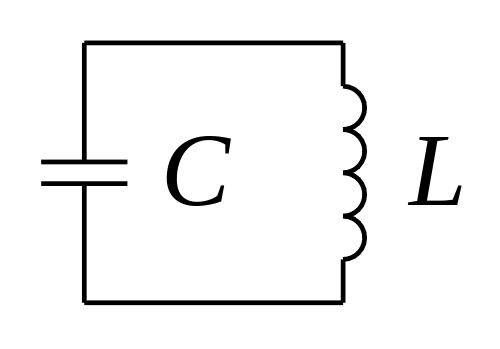
\includegraphics[scale=0.25]{500px-Schwingkreis.png}
\end{figure}
\begin{align*}
\text{Maschenregel} &\Rightarrow U(t)=L\dot{I}+\frac{Q}{C}=0 \\
&\stackrel{I=\dot{Q}}{\Rightarrow} L\ddot{Q}+\frac{Q}{C}=0 \\
&\Leftrightarrow \ddot{Q}+\underbrace{(\frac{1}{LC})}_{\omega_0^2}=0 \\
&\Rightarrow \omega_0=\frac{1}{\sqrt{LC}} 
\end{align*}
\end{document}